\documentclass[11pt]{beamer}
\usepackage[utf8]{inputenc}
\usepackage[T1]{fontenc}
\usepackage{lmodern}
\usepackage{amssymb}
\usepackage{pgfplots}
\usepackage{graphicx}
\usepackage{movie15}
\usepackage[french]{babel}
\usepackage{hyperref}
\usepackage{listings}

\usetheme{PaloAlto}

\addtobeamertemplate{footline}{\centering \insertframenumber/\inserttotalframenumber}

\begin{document}
	
\author[J.Delaeter C.Ghyselinck]{Joseph \bsc{Delaeter} et Corentin \bsc{Ghyselinck}}
\title{Projet Openxum}
\subtitle{Presentation orale 1}
\logo{
\includegraphics[width=45pt]{images/logo.jpg}}
\titlegraphic{
\includegraphics[width=50pt]{images/logo.jpg}}

  \begin{frame}[plain]
  \maketitle
  \end{frame}

  \begin{frame}
	\frametitle{Plan du cours}
	\tableofcontents
	\end{frame}
\section[Introduction]{Introduction}
  \begin{frame}
  \frametitle{Introduction}
  
  blablabla
  \end{frame}
\section[Description Jeux]{Descriptions Jeux} 
  \subsection[Dakapo]{Dakapo}
\begin{frame}
\frametitle{Dakapo}

\begin{columns}[T] % align columns
\begin{column}{.35\textwidth}
\color{red}\rule{\linewidth}{4pt}
 le jeu

\begin{center}
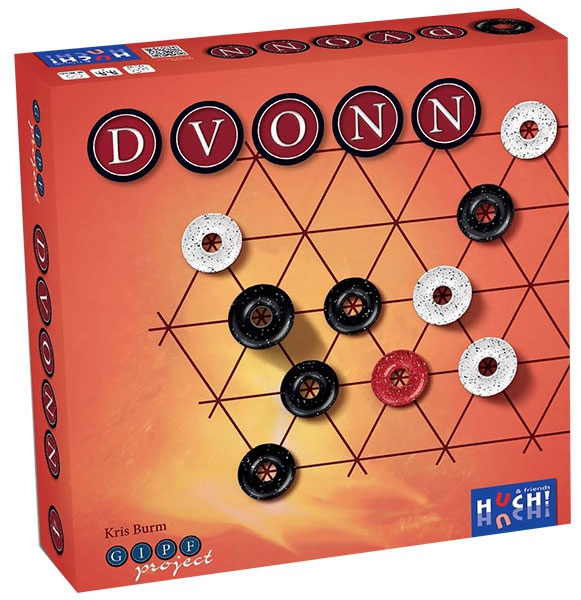
\includegraphics[width=100pt]{images/dvon.jpg}
\end{center}
\end{column}%

\hfill%
\begin{column}{.62\textwidth}
\color{blue}\rule{\linewidth}{4pt}
Description
\begin{itemize}
\item yolo 1
\item yolo 2
\item yolo 3
\end{itemize}
\end{column}%
\end{columns}

\end{frame}

\subsection[Hnefatafl]{Hnefatafl}
\begin{frame}
\frametitle{Hnefatafl}

\begin{columns}[T] % align columns
\begin{column}{.35\textwidth}
\color{red}\rule{\linewidth}{4pt}
 le jeu

\begin{center}
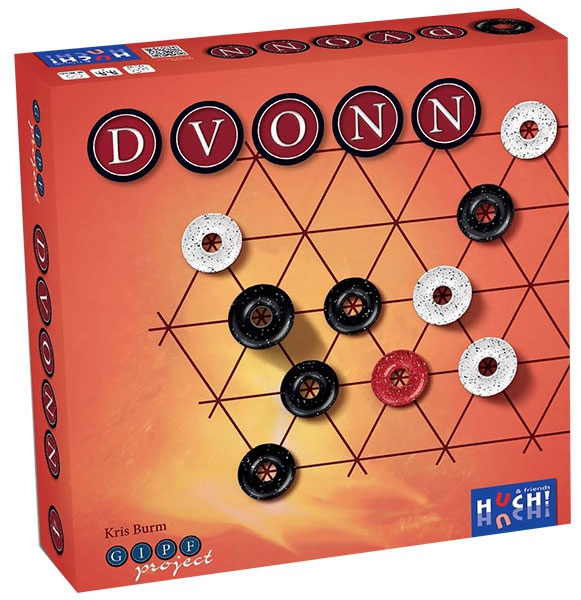
\includegraphics[width=100pt]{images/dvon.jpg}
\end{center}
\end{column}%

\hfill%
\begin{column}{.62\textwidth}
\color{blue}\rule{\linewidth}{4pt}
Description
\begin{itemize}
\item yolo 1
\item yolo 2
\item yolo 3
\end{itemize}
\end{column}%
\end{columns}

\end{frame}
\subsection[Kamisado]{Kamisado} 
\begin{frame}
\frametitle{Kamisado}

\begin{columns}[T] % align columns
\begin{column}{.35\textwidth}
\color{red}\rule{\linewidth}{4pt}
 le jeu

\begin{center}
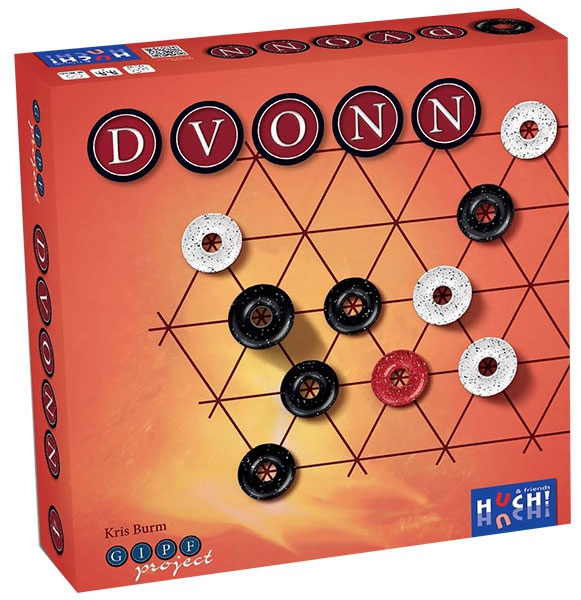
\includegraphics[width=100pt]{images/dvon.jpg}
\end{center}
\end{column}%

\hfill%
\begin{column}{.62\textwidth}
\color{blue}\rule{\linewidth}{4pt}
Description
\begin{itemize}
\item yolo 1
\item yolo 2
\item yolo 3
\end{itemize}
\end{column}%
\end{columns}

\end{frame}

\subsection[Neutreeko]{Neutreeko} 

\begin{frame}

\frametitle{Neutreeko}
\subtitle{Neutreeko}
\begin{columns}[t]
\begin{column}{3cm}
	\begin{block}{Plateau}
	\centering 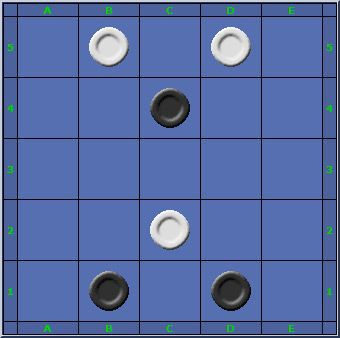
\includegraphics[width=80pt]{images/neut.jpg}
	\end{block} 
\end{column}

\begin{column}{7cm}
	\begin{block}{Regle}
		\begin{itemize}
			\item Noir qui commence. 
			\item Déplacement d'une  pièce dans la direction voulue.
			
			\item la pièce s'arrête si elle rencontre une autre pièce ou le bord du tablier. Il n'y a ni prise ni saut.
			
			\item Le but aligner ses trois pièces en continu.
		\end{itemize}
	\end{block}   
\end{column}
\end{columns}  
\end{frame}
%
%\begin{columns}[T] % align columns
%\begin{column}{.35\textwidth}
%\color{red}\rule{\linewidth}{4pt}
% le jeu
%
%\begin{center}
%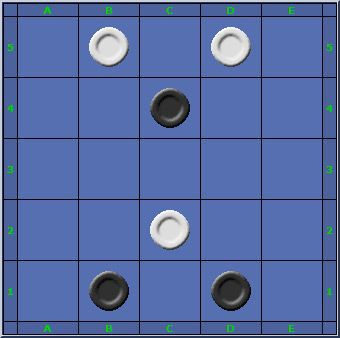
\includegraphics[width=70pt]{images/neut.jpg}
%\end{center}
%\end{column}%
%
%\hfill%
%\begin{column}{.62\textwidth}
%\color{blue}\rule{\linewidth}{4pt}
%Description
%\begin{itemize}
%\item Noir qui commence. 
%\item Déplacement d'une  pièce dans la direction voulue.
%
%\item la pièce s'arrête si elle rencontre une autre pièce ou le bord du tablier. Il n'y a ni prise ni saut.
%
%\item Le but aligner ses trois pièces en continu.
%\end{itemize}
%\end{column}%
%\end{columns}
   
\section{Pourquoi ces jeux?}  
  \begin{frame}
  \frametitle{Pourquoi ces 4 jeux?}

\begin{block}{ titre du block }
      Texte, équations, image, tableau etc ...
\end{block}

\begin{block}{ titre du block }
      Texte, équations, image, tableau etc ...
\end{block}

\begin{block}{ titre du block }
      Texte, équations, image, tableau etc ...
\end{block}
			
  \end{frame}
    
\section{IA}
\subsection{Alpha Beta Elagage} 
  \begin{frame}
  \frametitle{Elagage alpha beta}

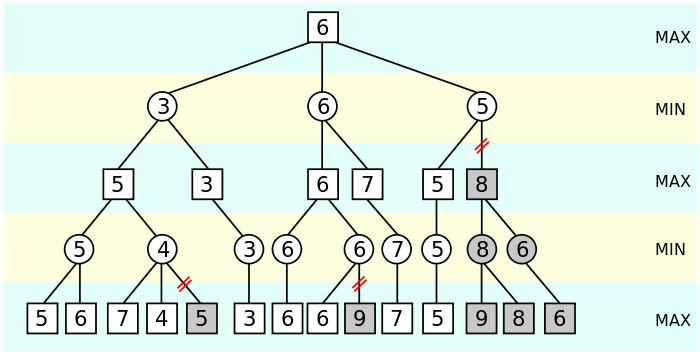
\includegraphics[width=150pt]{images/alphabeta.png}
  \end{frame}
 \subsection{MCTS}  
\begin{frame}
\frametitle{MCTS}
%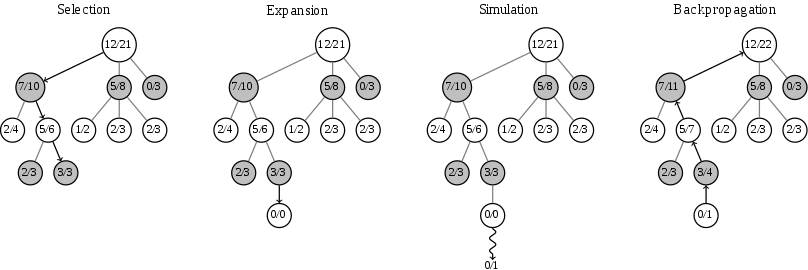
\includegraphics[width=340pt]{images/mcts.png}
\color{blue}\rule{\linewidth}{4pt}
Principe
\begin{itemize}
	\item yolo 1
	\item yolo 2
	\item yolo 3
\end{itemize}
Avantages
\begin{itemize}
	\item généralité
	\item calibrage
\end{itemize}
Limites
\begin{itemize}
	\item      coûteux
	\item non adapté aux jeux avec grand espace de recherche
\end{itemize}
  \end{frame}

\end{document}